% Architecture of reliable-tool-agent.
% Compile: pdflatex -interaction=nonstopmode architecture.tex   (one page sized to the drawing)
% PNG for the README, e.g.: pdftoppm -png -r 150 -singlefile architecture.pdf architecture
% Needs TikZ (Debian/Ubuntu: texlive-pictures). No `standalone` class, which lives in the
% much larger texlive-latex-extra: the page size is set with geometry instead.
%
% To mark a component as built, change its style from `planned=<colour>` to `built=<colour>`.

\documentclass{article}
\usepackage[paperwidth=16.4in, paperheight=9.4in, margin=0.3in]{geometry}
\pagestyle{empty}
\usepackage{tikz}
% Default Computer Modern sans serif: always installed (helvet needs extra font packages).
\renewcommand{\familydefault}{\sfdefault}
\usepackage{amssymb}
\usetikzlibrary{arrows.meta,calc}

\definecolor{app}{HTML}{4C72B0}
\definecolor{agent}{HTML}{DD8452}
\definecolor{guard}{HTML}{C44E52}
\definecolor{mcp}{HTML}{55A868}
\definecolor{data}{HTML}{8172B3}
\definecolor{ops}{HTML}{937860}

\tikzset{
  box/.style={rounded corners=5pt, align=center, font=\large, inner sep=3pt},
  % built=<colour>: coloured, solid border.
  built/.style={box, draw=#1, fill=#1!18, line width=1.1pt},
  % planned=<colour>: grey, dashed border (the colour is kept for when it gets built).
  planned/.style={box, draw=gray!65, fill=gray!6, dash pattern=on 4pt off 3pt,
                  text=black!65, line width=0.9pt},
  frametitle/.style={font=\Large\bfseries, text=black!75},
  arr/.style={-{Stealth[length=2.6mm]}, line width=0.9pt},
  darr/.style={{Stealth[length=2.6mm]}-{Stealth[length=2.6mm]}, line width=0.9pt},
  todo/.style={gray!65, dash pattern=on 4pt off 3pt},
  note/.style={font=\normalsize, text=black!65, align=center},
}

\begin{document}
\noindent
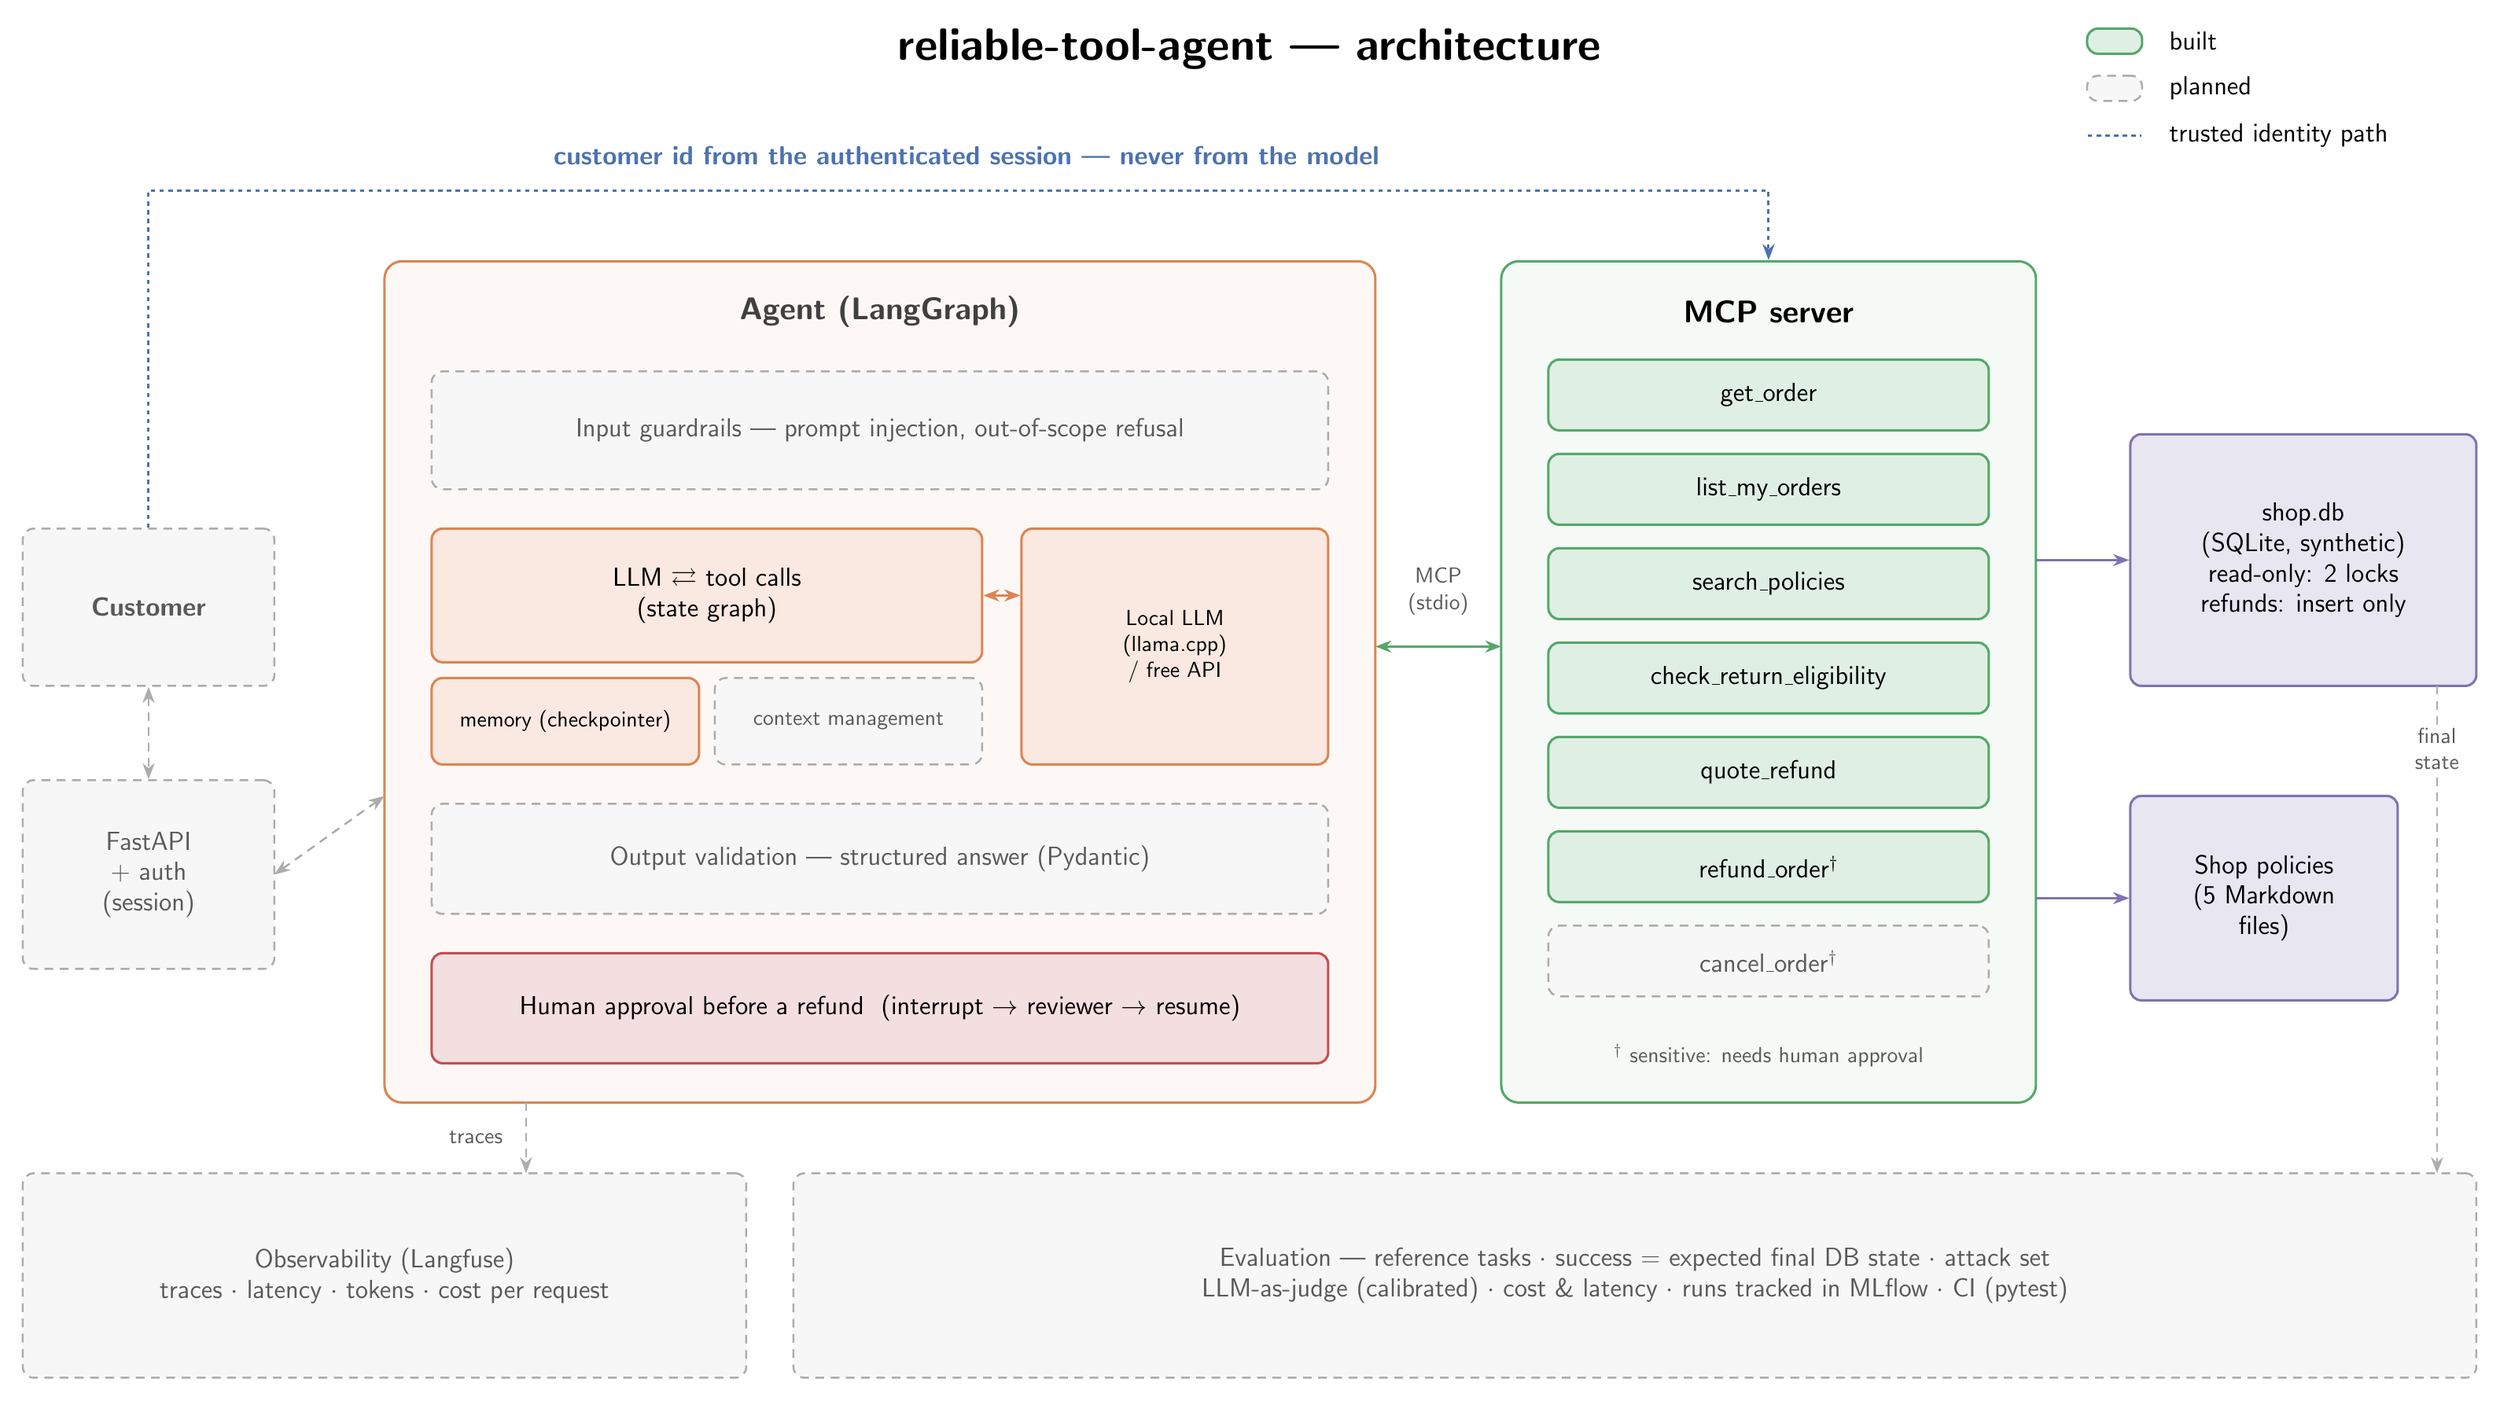
\begin{tikzpicture}[x=1in, y=1in]

  % Title
  \node[font=\huge\bfseries] at (8, 8.65) {reliable-tool-agent --- architecture};

  % ---------------------------------------------------------------- customer and API
  \node[planned=app, font=\large\bfseries, minimum width=1.6in, minimum height=1.0in]
    (customer) at (1.0, 5.1) {Customer};
  \node[planned=app, minimum width=1.6in, minimum height=1.2in]
    (api) at (1.0, 3.4) {FastAPI\\+ auth\\(session)};
  \draw[darr, todo] (customer.south) -- (api.north);

  % ---------------------------------------------------------------- agent
  \node[built=agent, fill=agent!6, minimum width=6.3in, minimum height=5.35in, rounded corners=8pt]
    (agent) at (5.65, 4.625) {};
  \node[frametitle] at (5.65, 6.98) {Agent (LangGraph)};
  \node[planned=guard, minimum width=5.7in, minimum height=0.75in]
    (guardin) at (5.65, 6.225) {Input guardrails --- prompt injection, out-of-scope refusal};
  \node[built=agent, minimum width=3.5in, minimum height=0.85in]
    (loop) at (4.55, 5.175) {LLM $\rightleftarrows$ tool calls\\(state graph)};
  \node[built=agent, font=\normalsize, minimum width=1.7in, minimum height=0.55in]
    (memory) at (3.65, 4.375) {memory (checkpointer)};
  \node[planned=agent, font=\normalsize, minimum width=1.7in, minimum height=0.55in]
    (context) at (5.45, 4.375) {context management};
  \node[built=agent, font=\normalsize, minimum width=1.95in, minimum height=1.5in]
    (llm) at (7.525, 4.85) {Local LLM\\(llama.cpp)\\/ free API};
  \node[planned=guard, minimum width=5.7in, minimum height=0.7in]
    (guardout) at (5.65, 3.5) {Output validation --- structured answer (Pydantic)};
  \node[built=guard, minimum width=5.7in, minimum height=0.7in]
    (hitl) at (5.65, 2.55)
    {Human approval before a refund \ (interrupt $\rightarrow$ reviewer $\rightarrow$ resume)};
  \draw[darr, agent] (loop.east) -- (llm.west |- loop.east);
  \draw[darr, todo] (1.8, 3.4) -- (2.5, 3.9);

  % ---------------------------------------------------------------- MCP server
  \node[built=mcp, fill=mcp!6, minimum width=3.4in, minimum height=5.35in, rounded corners=8pt]
    (mcp) at (11.3, 4.625) {};
  \node[frametitle, text=black] at (11.3, 6.98) {MCP server};
  \node[built=mcp,   minimum width=2.8in, minimum height=0.45in] at (11.3, 6.45) {get\_order};
  \node[built=mcp,   minimum width=2.8in, minimum height=0.45in] at (11.3, 5.85) {list\_my\_orders};
  \node[built=mcp,   minimum width=2.8in, minimum height=0.45in] at (11.3, 5.25) {search\_policies};
  \node[built=mcp,   minimum width=2.8in, minimum height=0.45in] at (11.3, 4.65) {check\_return\_eligibility};
  \node[built=mcp,   minimum width=2.8in, minimum height=0.45in] at (11.3, 4.05) {quote\_refund};
  \node[built=mcp,   minimum width=2.8in, minimum height=0.45in] at (11.3, 3.45) {refund\_order$^\dagger$};
  \node[planned=mcp, minimum width=2.8in, minimum height=0.45in] at (11.3, 2.85) {cancel\_order$^\dagger$};
  \node[note] at (11.3, 2.25) {$^\dagger$ sensitive: needs human approval};

  \draw[darr, mcp] (8.8, 4.85) -- (9.6, 4.85);
  \node[note] at (9.2, 5.2) {MCP\\(stdio)};

  % Trusted identity path: from the session to the tool server, around the model.
  \draw[app, line width=1.1pt, dash pattern=on 2pt off 2pt, -{Stealth[length=2.6mm]}]
    (customer.north) |- (11.3, 7.75) -- (mcp.north);
  \node[font=\large\bfseries, text=app] at (6.2, 7.97)
    {customer id from the authenticated session --- never from the model};

  % ---------------------------------------------------------------- data
  \node[built=data, minimum width=2.2in, minimum height=1.6in]
    (db) at (14.7, 5.4) {shop.db\\(SQLite, synthetic)\\read-only: 2 locks\\refunds: insert only};
  \node[built=data, minimum width=1.7in, minimum height=1.3in]
    (policies) at (14.45, 3.25) {Shop policies\\(5 Markdown\\files)};
  \draw[arr, data] (13.0, 5.4) -- (db.west);
  \draw[arr, data] (13.0, 3.25) -- (policies.west);

  % ---------------------------------------------------------------- observability, evaluation
  \node[planned=ops, minimum width=4.6in, minimum height=1.3in]
    (obs) at (2.5, 0.85)
    {Observability (Langfuse)\\traces $\cdot$ latency $\cdot$ tokens $\cdot$ cost per request};
  \node[planned=ops, minimum width=10.7in, minimum height=1.3in]
    (eval) at (10.45, 0.85)
    {Evaluation --- reference tasks $\cdot$ success = expected final DB state $\cdot$ attack set\\
     LLM-as-judge (calibrated) $\cdot$ cost \& latency $\cdot$ runs tracked in MLflow
     $\cdot$ CI (pytest)};

  % The agent emits traces; the evaluation checks the final state of the database.
  \draw[arr, todo] (3.4, 1.95) -- (3.4, 1.5);
  \node[note, anchor=east] at (3.3, 1.73) {traces};
  \draw[arr, todo] (15.55, 4.6) -- (15.55, 1.5);
  \node[note, fill=white, inner sep=1pt] at (15.55, 4.2) {final\\state};

  % ---------------------------------------------------------------- legend
  \begin{scope}[shift={(13.5, 8.2)}]
    \node[built=mcp, minimum width=0.35in, minimum height=0.16in] at (0, 0.5) {};
    \node[anchor=west, font=\large] at (0.3, 0.5) {built};
    \node[planned=mcp, minimum width=0.35in, minimum height=0.16in] at (0, 0.2) {};
    \node[anchor=west, font=\large] at (0.3, 0.2) {planned};
    \draw[app, line width=1.1pt, dash pattern=on 2pt off 2pt] (-0.17, -0.1) -- (0.17, -0.1);
    \node[anchor=west, font=\large] at (0.3, -0.1) {trusted identity path};
  \end{scope}

\end{tikzpicture}
\end{document}
